\chapter{Data and Methodology}
\label{chap:data_methodology}

This section details the data sources and methodological approaches employed in this thesis. It begins by describing the primary data source, the ICIJ Offshore Leaks Database (Section \ref{sec:3_1}), and the external datasets used for contextualization (Section \ref{sec:3_2}). Subsequently, it introduces a novel methodology utilizing agentic AI to enrich intermediary classification (Section \ref{sec:3_3}), outlines the general analytical methodologies applied (Section \ref{sec:3_4_analytical_methodologies}), and finally comments on the use of LLMs in the thesis preparation (Section \ref{sec:3_5_llms}).

\section{The ICIJ Offshore Leaks Database}
\label{sec:3_1}

The primary empirical basis for this thesis is the International Consortium of Investigative Journalists (ICIJ) Offshore Leaks Database. However, before detailing its structure, the inherent complexities and limitations associated with data derived from leaks concerning a domain deliberately designed for opacity will briefly be detailed.

\subsection{The Challenges of Obtaining and Interpreting Offshore Data}
\label{sec:data_challenges}

Researching the offshore financial system is inevitably difficult and fraught with challenges due to the pervasive secrecy that is its defining characteristic (Chang et al., 2023c; Christensen et al., 2022). The ICIJ database, while unparalleled in its scale and granularity, is not a comprehensive or randomly sampled representation of the entire offshore world. It is a compilation of data from specific leaks, each with its own origins and potential biases. For instance, a significant portion of the data originates from specific service providers like Mossack Fonseca (Panama Papers) or Appleby (Paradise Papers). Consequently, the observed patterns in clientele, jurisdictions, and service types may, to some extent, reflect the operational focus and market position of these particular firms rather than the offshore industry in its entirety (De Groen, 2017).

Hoang (2022) in her ethnography, notes of one of the ultra-wealthy board directors she interviews (FLAG: Ensure correct description), that despite the entities he was behind were revealed in the Panama Papers, nothing traces back to him. Instead, a group of "fall guys", as she terms them, are the ones that fall victim to the public's search-light. What we're dealing with in the ICIJ data is the comparatively more visible part of the long stem of offshore that's otherwise buried deep where no sunlight can act as Brandeis' disinfectant. 

An additional systematic bias arises from the inclusion of data from public corporate registries in certain jurisdictions as part of specific investigations (e.g., Paradise Papers incorporating registry data from Aruba, Bahamas, Barbados, Cook Islands, Lebanon, Malta, Nevis, and Samoa, as per the ICIJ `sourceID` variable). This data may include local businesses not engaged in typical offshore activities designed.

Nevertheless, despite these inherent limitations, the ICIJ Offshore Leaks Database represents the most extensive publicly available structured dataset on offshore entities and their associated actors. As Kejriwal \& Dang (2020, p. 3(FLAG: which page)) note: 

\begin{quote}
"[...] [P]recisely because the collection maps out a global system, the Panama Papers also present us with a golden opportunity to study the flow of information2 between firms, individuals and intermediaries. From a scientific perspective, the Panama Papers repre- sent a complex system, with entities that range from individuals to companies, many of which serve a specific purpose based on where in the world they are based, to a variety of relationships. Studying the structural properties of this complex system using applied networks science has the potential to reveal interesting trends about how such systems operate across geographies and economies."
\end{quote}

This thesis, therefore, acknowledges that it is analyzing the \textit{visible and structured tip of the iceberg}. Consequently, absolute counts or prevalence estimates for the entire offshore world derived from this data will likely be underestimates and must be interpreted with extreme caution. However, findings pertaining to the \textit{types} of activities, the \textit{characteristics} of observed actors (particularly intermediaries, who are often directly named), and the \textit{structural properties} of the revealed networks are more likely to offer robust, albeit partial, insights into the mechanisms of the offshore financial system. The use of the ICIJ database for such analytical purposes is increasingly established in academic research, with studies employing it to gauge propensities for offshore use (Alstadsæter et al., 2019; Londoño-Vélez \& Ávila-Mahecha, 2021) or to explore relationships between offshore structures and political contexts (Chang et al., 2023a; 2023b). This thesis will proceed with similar caution, focusing on patterns and relationships rather than definitive global estimates.

\subsection{Overview of the ICIJ Offshore Leaks Database}

Our primary dataset is the **International Consortium of Investigative Journalists (ICIJ) Offshore Leaks Database**. This publicly accessible repository is a comprehensive amalgamation of structured data meticulously extracted from several of ICIJ's landmark global investigations, most notably the Offshore Leaks (2013), Panama Papers (2016), Paradise Papers (2017/18), and Pandora Papers (2021/22). The database is substantial, cataloging information on over 810,000 offshore entities—which encompass a range of structures such as companies, trusts, and foundations—and establishing connections to more than 750,000 individuals and corporate entities. These connections span across a vast geographical landscape of over 200 countries and territories, with the underlying records covering a significant historical period, in some cases extending up to the year 2020.

\begin{figure}[htbp]
    \centering
    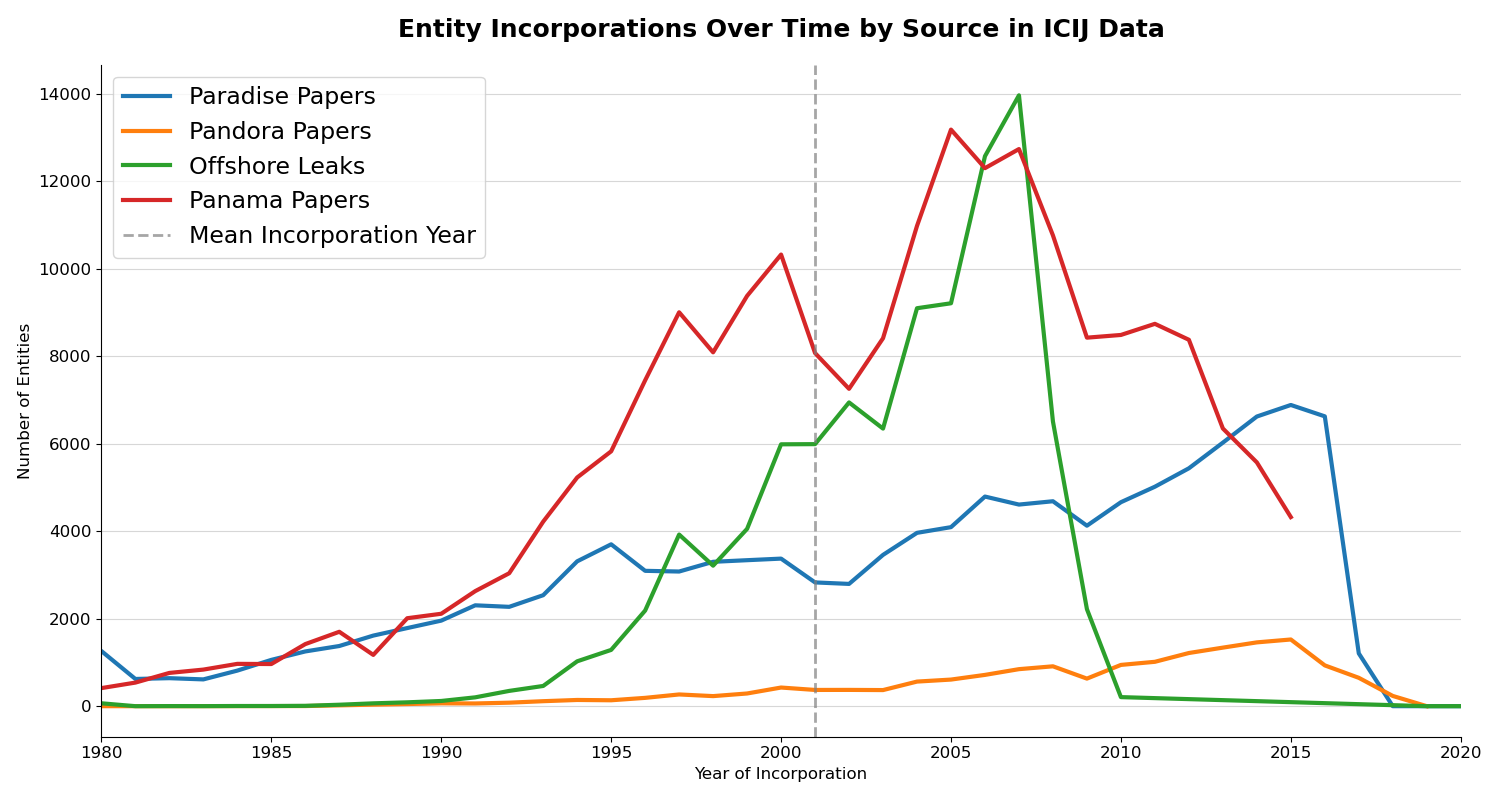
\includegraphics[width=0.8\textwidth]{Preliminary_Incorporations_over_Time.png}
    \caption{Overview of Entity Incorporations Over Time from ICIJ Data}
    \label{fig:incorporations_time}
\end{figure}
Before getting into the explanation, it is important to note that the overview provided here is relatively cursory and focuses mostly on the attributes and feature engineering specific to this thesis. For those more familiar with network analysis, I'd strongly encourage Kejriwal \& Dang's (2020) to get a more in-depth understanding of the data in more graph-theoretical terms.

The fundamental data model leveraged by the ICIJ data is a graph database. This model is used for its ability to represent interconnected information, conceptualizing data as \textbf{nodes} (the core informational units) and \textbf{edges} (the links defining how these units are connected). For the purposes of our study, the most pertinent node types are:
\begin{itemize}
    \item \textbf{Entities}: These represent the diverse offshore legal structures documented in the leaks, such as Limited companies, S.A. (Société Anonyme), Inc. (Incorporated), trusts, and foundations.
    \item \textbf{Officers}: This category includes individuals or, in some instances, other corporate bodies that fulfill specific roles (e.g., director, shareholder, beneficial owner, trustee, protector, nominee) within an Entity.
    \item \textbf{Intermediaries}: These are the professional facilitators—typically law firms, accounting practices, banks, trust companies, or specialized middlemen—who assist clients in the establishment and ongoing management of offshore entities. They often act as the liaison with offshore service providers like Mossack Fonseca or Appleby.
    \item \textbf{Addresses}: These nodes capture physical location data associated with the other node types, such as the registered office of an Entity or the business address of an Intermediary.
\end{itemize}

Relationships (edges) within this graph structure explicitly define the nature of the connections, for example, an Officer is an \texttt{officer\_of} an Entity, or an Intermediary acts as an \texttt{intermediary\_of} an Entity. The two primary node types of interest for this thesis are \textbf{Entities} and, critically, \textbf{Intermediaries}. In the ICIJ data model, the role of intermediaries is, with very few exceptions, represented entirely through their connections to Entities. That is, at a high level, a common relational pathway is: Intermediaries are \texttt{intermediary\_of} Entities, which in turn have Officers (who are \texttt{officer\_of} these Entities).

\subsection{Entities}

Delving deeper into the \textbf{entities}, the information processed from source files such as \texttt{nodes-entities.csv} and \texttt{relationships.csv} provides a rich set of attributes for each. Key data points include the entity's registered \texttt{name}, its \texttt{jurisdiction} of incorporation (which is standardized to ISO3 country codes for consistent geographical analysis), and the \texttt{country\_codes} associated with its operational activities or linked addresses. These \texttt{country\_codes} are often distinct from its legal \texttt{jurisdiction} of incorporation and provide insights into the geographical footprint of the entity's actual business or connections. Further attributes encompass the \texttt{incorporation\_date}, its operational \texttt{status} (e.g., Active, Struck Off, Dissolved), and its specific \texttt{entity\_type} (e.g., Standard International Company, Trust, Business Company Limited by Shares).

A particularly significant feature derived for each entity is the \texttt{bearer\_count}. This metric quantifies the number of associated officers explicitly identified as "Bearer" or its linguistic equivalents (e.g., "THE BEARER," "EL PORTADOR"), which are standardized from variations found in the \texttt{officers\_df}. The presence of bearer instruments, as highlighted by Harrington (2016), is a critical indicator of mechanisms used to obscure true beneficial ownership. In such arrangements, legal ownership follows the physical possession of the share certificate rather than being recorded in a central register, thereby enhancing anonymity (Chang et al., 2023c).

\subsection{Intermediaries and Feature Engineering}

For \textbf{intermediaries}, whose foundational data is drawn from \texttt{nodes-intermediaries.csv}, the analysis extends beyond basic identifying information. Beyond their \texttt{name} and the \texttt{countries} associated with their operational addresses, we calculate their \texttt{degree}. In this context, the degree represents the total number of distinct entities an intermediary is connected to within the ICIJ network, serving as a proxy for their client base size or activity level.

More extensively, we construct several aggregated metrics that characterize each intermediary based on the collective properties of the entities they service. As our primary research interest lies in understanding the roles and specializations of intermediaries, we aggregate information at the intermediary-level about the entities they are connected to. While graph data models excel at representing complex, interrelated data, extracting features for broader statistical analysis often necessitates such aggregation into key-value attributes (Kejriwal \& Dang, 2020).

For every intermediary, we generate the following features:

\begin{itemize}
   \item \texttt{country\_counts}: A dictionary detailing the frequency of entities they are connected to, grouped by the \texttt{country\_codes} associated with those entities. This reflects the geographical spread of the operational links of the entities they service. The derivation of these \texttt{country\_codes} from address fields in the original leaks means their completeness and precision can vary, a factor considered in interpreting derived metrics.
   \item \texttt{jurisdiction\_counts}: A dictionary detailing the frequency of entities they are connected to, grouped by the \texttt{jurisdiction} (ISO3 code) in which those entities are incorporated. This captures the intermediary's usage of different offshore legal environments.
   \item \texttt{regime\_counts}: A dictionary detailing the frequency of entities they are connected to, grouped by the political regime type (e.g., Liberal Democracy, Closed Autocracy, as per VDem data detailed in Section \ref{sec:3_2}) of the entities' associated \texttt{country\_codes} at the time of entity incorporation. This provides insight into the political contexts linked to an intermediary's client base. Note, VDem do not classify a lot of those countries that are tax havens (e.g. Bahamas, British Virgin Islands etc.), because their methodology is not robust to these countries that are as small (FLAG: Find that appendix in VDem). For the sake of this thesis, when the VDem data cannot be matched, we assign the regime type as "Microstate".
   \item \texttt{legal\_tech\_counts}: A dictionary detailing the frequency of entities they are connected to, grouped by the predominant types of "legal technologies" (e.g., Banking, Corporate, Dual-Purpose, as per Laffitte (2024), detailed in Section \ref{sec:3_2}) prevalent in the entities' jurisdictions of incorporation at the time of their formation. This reflects an intermediary's engagement with specific offshore legal architectures.
\end{itemize}

Furthermore, we quantify for each intermediary the number of entities they are connected to that have \texttt{bearers\_connected} (i.e., entities with a \texttt{bearer\_count} > 0) and calculate the \texttt{bearer\_share}, representing the proportion of their serviced entities that utilize these anonymity-enhancing instruments.

To measure the diversity of their client entity portfolio across these dimensions, we also compute normalized entropy scores: \texttt{country\_entropy}, \texttt{jurisdiction\_entropy}, \texttt{regime\_entropy}, and \texttt{legal\_tech\_entropy}. More on that in Section \ref{subsec:entropy}. These scores provide a measure of the diversity of the intermediary's client base across the respective dimensions, with higher values indicating a more diverse portfolio.

\section{Other Data Sources}
\label{sec:3_2}
To enrich the core ICIJ data, several external datasets are integrated, primarily to provide contextual information at the country or jurisdiction level, and to classify intermediaries by type.

\begin{itemize}
    \item \textbf{Laffitte Legal Technologies Data (HTHD)}: This dataset (Laffitte, 2024) is used for connecting historical legal framework changes to entities and their structuring, specifically identifying the "legal technologies" active in a jurisdiction at the time of an entity's incorporation.
    \item \textbf{VDem (Varieties of Democracy) Data}: This provides country-level variables, notably political regime types, for the jurisdictions and countries associated with entities and intermediaries.
    \item \textbf{Intermediary Type Enrichment}: As detailed in Section \ref{sec:3_3_agentic_ai_classification} (updated label), an agentic AI approach is employed to classify a subset of intermediaries based on publicly available information scraped from the internet.
\end{itemize}

\section{Other Data Sources}
\label{sec:3_2}
To enrich the core ICIJ data, several external datasets are integrated, primarily to provide contextual information at the country or jurisdiction level, and to classify intermediaries by type.

\begin{itemize}
    \item \textbf{Laffitte Legal Technologies Data (HTHD)}: This dataset (Laffitte, 2024) is used for connecting historical legal framework changes to entities and their structuring, specifically identifying the "legal technologies" active in a jurisdiction at the time of an entity's incorporation.
    \item \textbf{VDem (Varieties of Democracy) Data}: This provides country-level variables, notably political regime types, for the jurisdictions and countries associated with entities and intermediaries.
    \item \textbf{Intermediary Type Enrichment}: As detailed in Section \ref{sec:3_3}, an agentic AI approach is employed to classify a subset of intermediaries based on publicly available information scraped from the internet.
\end{itemize}

At the country and jurisdiction level, we utilize data from the Varieties of Democracy (VDem) project for information on political regime types, and Sébastien Laffitte's (2024) Historical Tax Havens Database (HTHD), developed for his doctoral thesis, which provides detailed information on the evolution of legal technologies in various jurisdictions.

\begin{enumerate}
  \item The \textbf{Varieties of Democracy (VDem) Project data} (specifically \texttt{vdem\_core.csv}): We utilize the \texttt{v2x\_regime} variable from VDem's comprehensive dataset to enrich our entity data. This variable classifies countries into categories such as Closed Autocracy, Electoral Autocracy, Electoral Democracy, or Liberal Democracy. By matching an entity's associated \texttt{country\_codes} (representing operational links) and its \texttt{incorporation\_year} with the VDem data for the corresponding country and year, we assign a political regime classification to each entity. This entity-level regime information is then aggregated to construct the \texttt{regime\_counts} at the intermediary level, providing insight into the political environments linked to an intermediary's clientele.
  
  \item \textbf{Laffitte's (2024) "The Market for Tax Havens" dataset} (specifically \texttt{HTHD.csv}): This dataset offers a historical perspective on the "offshore legal architecture" of various jurisdictions, detailing their adoption of different "legal technologies" such as International Business Company (IBC) laws, trust legislation, or banking secrecy provisions. Laffitte categorizes these into broader types such as "Banking," "Corporate," "Dual-Purpose" (e.g., IBCs serving both personal and corporate needs), and "Personal" (e.g., trust laws). We merge this dataset onto our entity data by matching the entity's \texttt{jurisdiction} of incorporation and its \texttt{incorporation\_year} with the HTHD data. This allows us to identify the specific legal technologies active in an entity's jurisdiction at its time of incorporation. This entity-level characterization is subsequently aggregated to create the \texttt{legal\_tech\_counts} at the intermediary level, reflecting the types of legal environments their serviced entities operate within.
\end{enumerate}

\section{Agentic AI for Intermediary Classification}
\label{sec:3_3}

Directly at the Intermediaries-level, we also enrich a \textbf{subset of intermediaries} (specifically, a random sample of 500 and the top $\sim$1.5\% by degree, chosen to balance representativeness with computational feasibility for the AI agent) with information on their specific "type." This classification is based on a typology adapted from the EU (2017) report on the Panama Papers (De Groen, 2017), which identifies roles such as Tax Expert, Legal Expert, Administrator, and Investment Advisor.

The core idea is to use an AI agent loop to automate the process of gathering information about and classifying the intermediaries listed in the ICIJ data. The basic workflow is illustrated in Figure \ref{fig:agent_loop_placeholder}.

\begin{figure}[htbp]
    \centering
    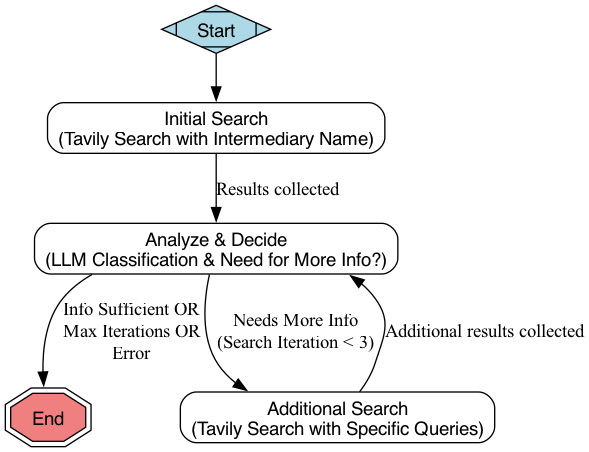
\includegraphics[width=0.8\textwidth]{Methods_Agent_Graph.png}
    \caption{Agent Setup for Intermediary Classification}
    \label{fig:agent_loop_placeholder}
\end{figure}

In brief, the process involves an AI agent orchestrating online searches for each intermediary identified in the ICIJ data. It begins with generic searches, reads and interprets the initial results, and then formulates more specific search queries based on the information discovered or identified as lacking. This iterative process involves up to three search queries per intermediary, scouring the top 15 most relevant web results identified through query-result embedding similarity using the Tavily Search API (though the tool is relatively generic and its specific choice is not critical to the methodology). This effectively replaces the time-consuming need for manual searching of the intermediaries.

Based on the information gathered, the AI agent then classifies the intermediary according to the De Groer (2017) typology (Tax Expert, Legal Expert, Administrator, Investment Advisor), adding a few additional relevant fields (e.g., specific job title). To mitigate some of the obvious fallibility of such an enrichment method, the agent also provides a confidence score for its classification judgment, which is filtered on in the analysis.


\section{Analytical and Statistical Techniques Applied}
\label{sec:3_3_analytical_methodologies}

This section outlines the core analytical techniques applied to the processed data, with a primary emphasis on concepts from network theory for characterizing the structure of the ICIJ data. These network methods are central to the thesis, while other approaches, such as unsupervised learning for pattern discovery and statistical tests for assessing significance, serve as ancillary tools and will be discussed more briefly.

\subsection{Concepts from Network Analysis}
\label{subsec:network_theory_concepts}

The application of network analysis is fundamental to this thesis, drawing on a tradition of using such methods to understand the nature of complex, often covert or illicit, systems (Morselli, 2009). Specifically, network analysis is employed here to uncover the roles intermediaries play based on their positions within the interconnected offshore financial system revealed by the ICIJ data. As described in Section \ref{sec:3_1}, the ICIJ data forms a multi-modal graph (comprising entities, officers, intermediaries, etc.). Directly applying many standard network analysis concepts to such a multipartite graph can be challenging. Therefore, our approach often involves analyzing specific projections or subsets of the global graph to make the analytical tools from network theory applicable. The foundational textbook by Newman (2010) serves as the primary reference for this section.

\begin{itemize}
    \item \textbf{Centrality Scores}: To identify nodes of critical importance within specific network representations, we utilize two fundamental centrality measures. In the context of understanding the key countries for intermediary activity, these measures are applied to a network derived from intermediary incorporation patterns.
    \begin{itemize}
        \item \textbf{Eigenvector Centrality}: This measure assigns scores to nodes based on the principle that connections to high-scoring nodes contribute more to the score of the node in question than equal connections to low-scoring nodes. It is calculated as the principal eigenvector of the adjacency matrix $\mathbf{A}$ of the network, satisfying $x_i = \frac{1}{\lambda} \sum_{j} A_{ij} x_j$, where $x_i$ is the centrality score of node $i$, $A_{ij}$ is 1 if node $i$ is connected to node $j$ and 0 otherwise (or the weight of the edge), and $\lambda$ is the largest eigenvalue of $\mathbf{A}$ (cf. Perron-Frobenius theorem). Eigenvector centrality is chosen for its ability to identify nodes that are influential not just by having many connections, but by being connected to other influential nodes, providing a robust reading of which countries are most central in the network of intermediary incorporations.
        \item \textbf{Betweenness Centrality}: This metric quantifies the extent to which a node lies on shortest paths between other pairs of nodes. For a node $v$, it is defined as $C_B(v) = \sum_{s \neq v \neq t} \frac{\sigma_{st}(v)}{\sigma_{st}}$, where $\sigma_{st}$ is the total number of shortest paths between nodes $s$ and $t$, and $\sigma_{st}(v)$ is the number of those paths that pass through $v$. Betweenness centrality is used here to gauge which countries act as crucial "bridges" or conduits within the network, potentially connecting otherwise disparate segments, a role distinct from simply being a high-degree hub.
    \end{itemize}

    \item \textbf{Community Detection: Modularity Maximization}: To uncover clusters or communities of closely related nodes within the country network, we employ modularity maximization. This approach provides an atheoretical method for identifying densely connected groups of countries, which may reflect underlying similarities in how intermediaries utilize them. Such clustering could be influenced by factors like shared regime types (Chang et al., 2023c) or the trust dynamics inherent in relational capitalism. While traditional clustering algorithms could be applied, defining a meaningful distance or dissimilarity metric for nodes in these networks is non-trivial. Modularity maximization, conversely, assesses the quality of a partition by comparing the number of intra-community edges to what would be expected in a random network with similar properties (a null model). The quality of a partition $C$ is measured by the modularity $Q$:
    \begin{equation}
        Q = \frac{1}{2m} \sum_{i,j} \left[ A_{ij} - P_{ij} \right] \delta(c_i, c_j)
    \end{equation}
    where $m$ is the total number of edges, $A_{ij}$ is the actual weight of the edge between nodes $i$ and $j$, $P_{ij}$ is the expected weight of an edge between $i$ and $j$ under the Newman-Girvan null model (a configuration model preserving the degree sequence, where $P_{ij} = \frac{k_i k_j}{2m}$ for unweighted graphs, $k_i$ being the degree of node $i$), and $\delta(c_i, c_j)$ is 1 if nodes $i$ and $j$ are in the same community ($c_i=c_j$) and 0 otherwise. Since finding the optimal partition is an NP-hard (although, to be honest, at the size we reduce our graph sizes, search space isn't an issue...) problem, we utilize the Louvain method (Blondel et al., 2008), an efficient and widely adopted greedy algorithm, as implemented in the \texttt{networkx} library.

    \item \textbf{Power-law Distribution}: The distribution of node degrees (number of connections) and other network properties are examined for characteristics of power-law distributions. A power law, $P(k) \sim k^{-\alpha}$, describes a "fat-tailed" distribution where a few nodes (hubs) have a disproportionately high number of connections, while most nodes have few. Such distributions are frequently observed in real-world networks (Clauset et al., 2009; Kejriwal \& Dang, 2020) and their presence can indicate significant heterogeneity in node importance.

    \item \textbf{Density of a Graph}: Network density, the ratio of actual edges to the total number of possible edges in the network ($D = \frac{L}{N(N-1)/2}$ for an undirected graph with $L$ edges and $N$ nodes), is used to measure the general level of connectedness. Low density is typical for large, sparse networks and indicates that connections are selective rather than ubiquitous.
\end{itemize}

\subsection{Entropy}
\label{subsec:entropy}
Drawing on its application in prior studies of offshore finance (e.g., Chang et al., 2023c; Kejriwal \& Dang, 2020), Shannon entropy is employed as a measure of diversity or concentration. For a discrete random variable $X$ with $n$ possible outcomes $x_1, ..., x_n$ and probabilities $p(x_i)$, entropy is defined as:
\begin{equation}
    H(X) = -\sum_{i=1}^{n} p(x_i) \log_b p(x_i)
\end{equation}
where $b$ is the base of the logarithm (typically $b=2$, yielding units of bits). Compared to other concentration measures like the Herfindahl-Hirschman Index (HHI), entropy gives more weight to smaller amounts of diversity. This characteristic is particularly useful in this thesis, as intermediaries' activities (e.g., choice of jurisdictions or countries) are often highly concentrated in one or two locations, but variations in minor activities can still be informative. Normalized entropy, calculated by dividing $H(X)$ by the maximum possible entropy ($\log_b n$), is used to provide a standardized measure (0 to 1) for comparing diversity across intermediaries with different breadths of activity. Entropy is used, for example, as a summary statistic at the intermediary-level to quantify the diversity of their client entity portfolio across dimensions like country, jurisdiction, or regime type, enabling subsequent comparisons of these distributions across different intermediary classifications.

\subsection{Association Analysis}
\label{subsec:unsupervised_learning}
In line with the highly exploratory nature of this thesis, unsupervised learning techniques are employed to discover notable patterns within the data. Association analysis (Hastie et al., 2009) is particularly opportune for identifying non-obvious relationships or co-occurrences in large datasets, such as the ICIJ networks. For example, it can help determine which connections (e.g., between a type of intermediary and the use of a specific jurisdiction or legal technology) are particularly remarkable. This approach relies on a \textbf{non-parametric notion} of pattern discovery, aiming to \textbf{discover patterns of high density} or co-occurrence.

Two main tools from association analysis, based on simple set-theoretical notions, are used:
\begin{itemize}
    \item \textbf{Support}: This measures the overall frequency of an itemset (e.g., a specific attribute or combination of attributes) in the dataset. For an itemset $X$, $Support(X) = P(X) = \frac{\text{count}(X)}{N}$, where $N$ is the total number of transactions (e.g., intermediaries). For an association rule $A \rightarrow B$, $Support(A \rightarrow B) = P(A \cup B)$.
    \item \textbf{Lift}: This measures how much more likely item $B$ is to be present when item $A$ is present, compared to the baseline probability of $B$. It indicates the strength of an association beyond what would be expected by chance.
    \begin{equation}
        Lift(A \rightarrow B) = \frac{P(B|A)}{P(B)} = \frac{Support(A \cup B)}{Support(A) \times Support(B)}
    \end{equation}
    A lift value greater than 1 suggests a positive association, a value less than 1 suggests a negative association, and a value of 1 suggests independence. \textbf{Lift scores} will be used to quantify the strength of associations found, indicating, for example, how much more likely an intermediary of a certain type is to use a specific jurisdiction compared to the overall likelihood.
\end{itemize}

\subsection{Multiple Hypothesis Testing}
\label{subsec:multiple_hypothesis_testing}
Given that this thesis is highly exploratory and investigates a multitude of potential associations, it is crucial to address the issue of multiple hypothesis testing. When numerous statistical tests are performed, the conventional Type I error rate of 5\% ($p < 0.05$) can become inflated, leading to a higher probability of false positives (incorrectly rejecting a true null hypothesis). To counteract this, a highly conservative approach is adopted, opting for the \textbf{Bonferroni correction} to control the Family-Wise Error Rate (FWER) at the conventional maximum of 5\%. This method adjusts the significance threshold for each individual test to $\alpha/m$, where $\alpha$ is the desired FWER (e.g., 0.05) and $m$ is the total number of hypotheses tested. Alternatively, individual p-values are multiplied by $m$, and then compared to $\alpha$. While known for its conservatism, this choice is made to be particularly cautious about any single false positive claim, given the exploratory nature of the analysis, rather than opting for procedures like the Benjamini-Hochberg method which control the False Discovery Rate (FDR).

\subsection{Testing Significance of Results}
\label{subsec:significance_testing}
In line with the considerations above, and the nature of the data, specific non-parametric statistical tests are employed to assess the significance of observed differences or associations. These tests are chosen for their robustness to violations of normality assumptions. The following are applied where appropriate, with detailed applications described in the empirical analysis chapter:
\begin{itemize}
    \item \textbf{Mann-Whitney U test}: A non-parametric test used for comparing the distributions of continuous or ordinal variables between two independent groups. It is particularly useful when the data is not normally distributed, as is often the case with metrics like entropy scores or network-derived measures. It assesses whether one distribution is stochastically greater than the other.
    \item \textbf{Fisher's exact test}: Employed for analyzing categorical data, particularly in contingency tables (e.g., 2x2 tables). This test is ideal for assessing associations between categorical variables, such as those resulting from association analysis or when examining the relationship between dummy variables (e.g., whether entities are connected to bearer instruments and intermediary type). It is an exact test, making it suitable for small sample sizes or when expected cell counts are low.
    \item \textbf{Two-sample Kolmogorov-Smirnov test}: Used for comparing the underlying distributions of continuous variables from two independent samples. Unlike tests that compare central tendencies (like the t-test or Mann-Whitney U), the K-S test is sensitive to differences in location, scale, and shape of the distributions, offering a more comprehensive comparison.
\end{itemize}


\section{Use of LLMs in the Broader Paper}
\label{sec:3_5_llms}

LLMs have also been used to polish the text of this thesis and used for idea generation.

Used Google Gemini models mainly.
\begin{itemize}
    \item gemini-2.5-pro-preview-05-06
    \item gemini-2.5-pro-experimental-03-25
    \item gemini-2.5-flash-experimental-04-17
\end{itemize}

Quick edits frequently made using Claude's 3.7 Sonnet model (`claude-3.7-sonnet-latest`).



